\documentclass{article}
\usepackage[utf8]{inputenc}
\usepackage{amsmath}
\usepackage{amssymb}
\usepackage{graphicx}
\usepackage{epstopdf}
\usepackage{geometry}
\usepackage{url}
\usepackage{float}
\usepackage{array}
\usepackage[export]{adjustbox}

\usepackage{todonotes}
\usepackage{bytefield}


\usepackage{enumitem}

\newlist{registerdescription}{description}{2}
\setlist[registerdescription]{labelwidth=1.5cm,leftmargin=!,font=\normalfont}

\usepackage{geometry}
 \geometry{
   a4paper,
   total={170mm,257mm},
   left=30mm,
   right=30mm,
   top=15mm,
 }

\title{Embedded Systems Mini-Project\\
 Avalon Camera Controller Implementation on Cyclone V FPGA}
\author{
  Snoeijs, Jan\\
  EPFL\\
  \texttt{jan.snoeijs@epfl.ch}
  \and
  Spieler, Michael\\
  EPFL\\
  \texttt{spieler.micheal@epfl.ch}
  }

\date{January 2018}

\begin{document}

\maketitle

\section{Introduction}
In this document we present our implementation of the design proposed in our report of laboratory 3, on the Cyclone V FPGA using a NIOS II processor and an Avalon Bus. We will more specifically detail the changes we made compared to the theoretical design and explain the structure of our VHDL and software source files, as well as the top-level Qsys connectivity.

\section{Hardware structure}

In this section we present the hardware structure of our implemented design and compare the small differences with the theoretical design.

\subsection{Custom Component: Avalon Camera Controller}

The implemented hardware architecture of the custom camera controller is shown in Figure \ref{fig:CameraComponent}. We made some changes compared to the theoretical version of the design; specifically, we added (green) and removed (red) some top-level connections, put the LineFIFO out of the Camera Interface component and the PLL outside our Custom Component (connected as an additional component in Qsys). These changes are induced by the hierarchy we chose for our VHDL files, and for simplicity the routing of all internal components was done in our custom component top-level file. Concerning the PLL, we removed it from our component because its clock output was always zero if we integrated it.

\begin{figure}[H]
\centering
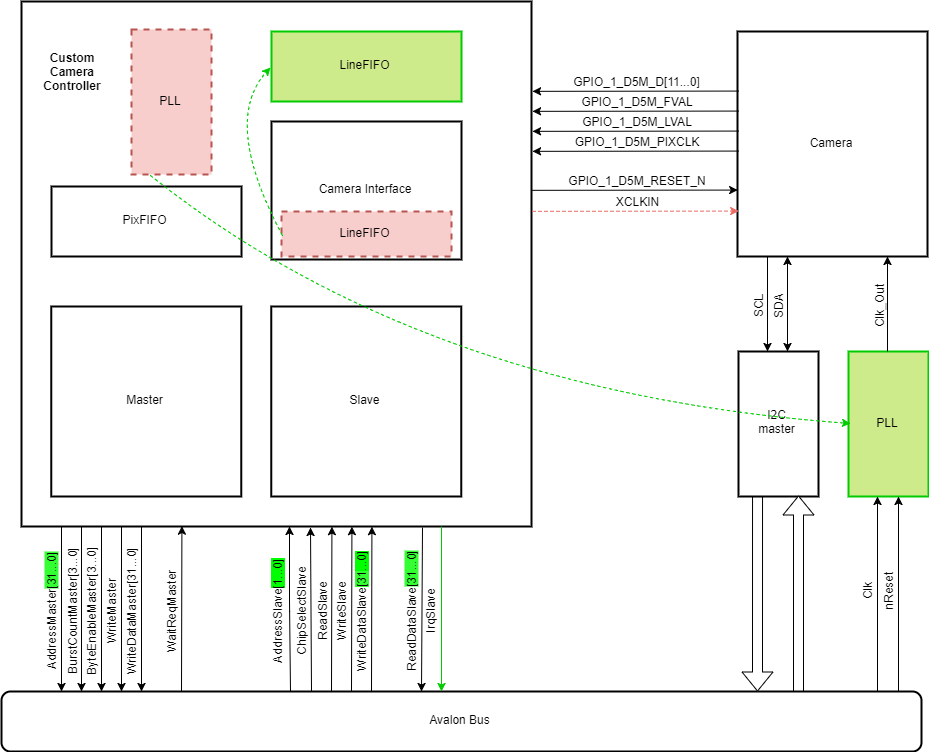
\includegraphics[scale=0.4]{images/CameraComponent.png}
\caption{Custom avalon camera controller --- Implemented architecture and modifications}
\label{fig:CameraComponent}
\end{figure}

\subsection{Integration of Custom Component in FPGA}

Figure \ref{fig:FpgaSystem} shows the full system architecture implemented on the Cyclone V FPGA.

\begin{figure}[H]
\centering
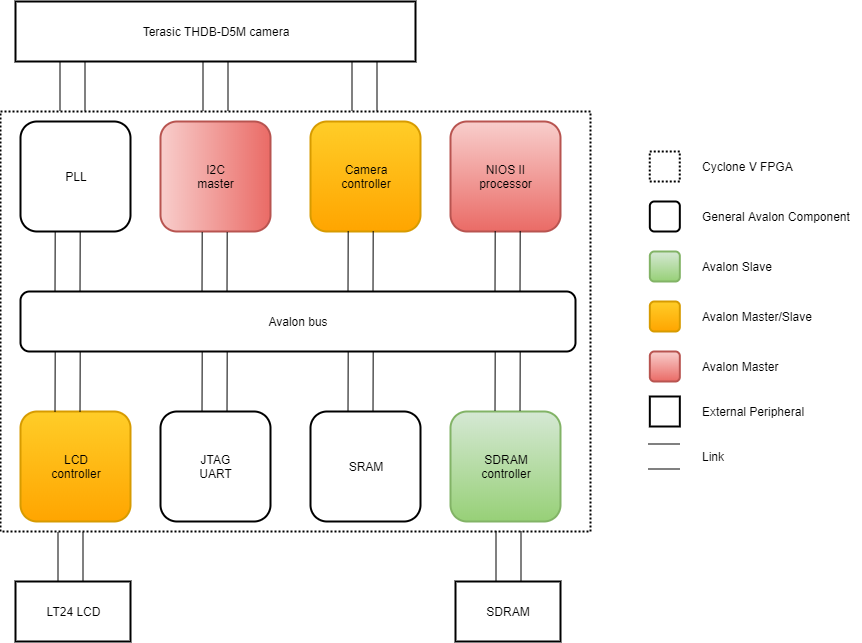
\includegraphics[scale=0.45]{images/FpgaSystem.png}
\caption{FPGA Full System Architecture --- Implementation on Cyclone V}
\label{fig:FpgaSystem}
\end{figure}

\section{Hardware Implementation}

We present the detailed implementation of the hardware architecture shown in the previous section. 

\subsection{Avalon Slave Component}
\todo[inline]{
Removed the ImaageStart Interrupt \\
Removed MasterEnable signals \\
Image Address can be updated anytime, will be applied for next image. \\
}

\subsection{Camera Controller Component}
\todo[inline]{
Removed the down sampling. The camera already sends a correct image size. \\
}
\subsection{Avalon Master component}

The master component reads the data from the dual-clocked PixFIFO and writes in the SDRAM through burst transfers on the Avalon bus. The slave component transmits the memory address of the start of the image. During one burst, 8 32-bit words are sent sequentially to the memory. The component's behavior is controlled by a tri-state FSM which generates the necessary Avalon signals which are necessary for a burst transfer. For example, the outputting of the Avalon address and the dependency to input signal \verb'waitreq' are handled by this state machine. 

\begin{figure}[H]
\centering
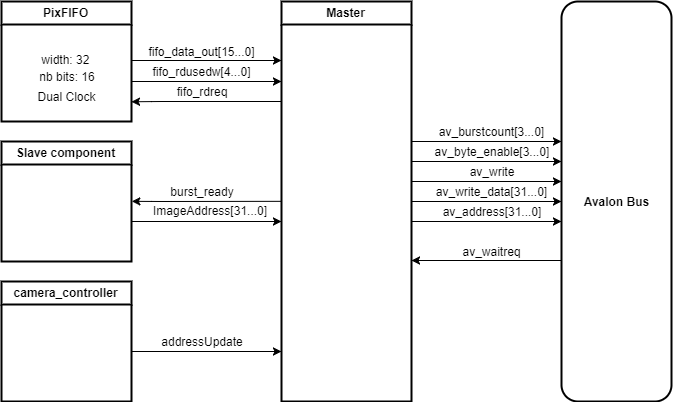
\includegraphics[scale=0.6]{images/MasterGeneral.png}
\caption{Master component --- Interconnects}
\label{fig:MasterGeneral}
\end{figure}

\subsubsection{Finite state machine description}

The FSM is in \verb'IDLE' state until the PixFIFO (32 x 16-bits) gets filled with atleast 16 pixels (16 lines of 16 bits). Between the theoretical design and the implementation we chose to increase the width of the PixFIFO. In the implementation, the state machine is triggered by the \verb'rdusedw[4...0]' signal instead of by the \verb'fifo_full' signal, which should be more robust to data losses in cases of a long wait time on the avalon side. An extra state was added to the finite state machine so that the data transfers in a bursts are consecutive and not interrupted by a processing cycle as that would have been the case with only 2 states. In fact, in the theoretical design we overlooked the fact that only one 16-bit data is available at the same time at the output of the FIFO. Thus the added state (\verb'STORE') actually stores the data contained in the FIFO into a register where all the data is available in parallel. We unfortunately first wrote the master VHDL before realizing that the data can have a different format at the input and output of an Altera FIFO, which would have saved us some logic in the master component. Nevertheless, our implementation of this logic should be functionally correct. Finally the \verb'WRITE' is the state in which the burst transfers are executed and is similar to the one presented in the theoretical design.

\begin{figure}[H]
\centering
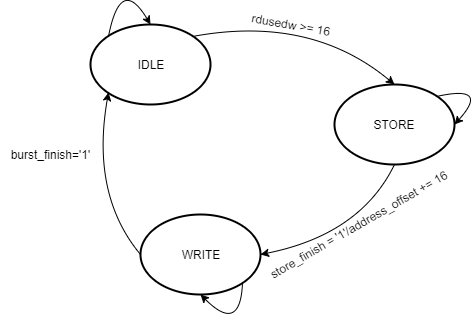
\includegraphics[scale=0.45]{images/MasterFSM.png}
\caption{Master component --- Modified finite state machine}
\label{fig:MasterFSM}
\end{figure}

\begin{figure}[H]
\centering
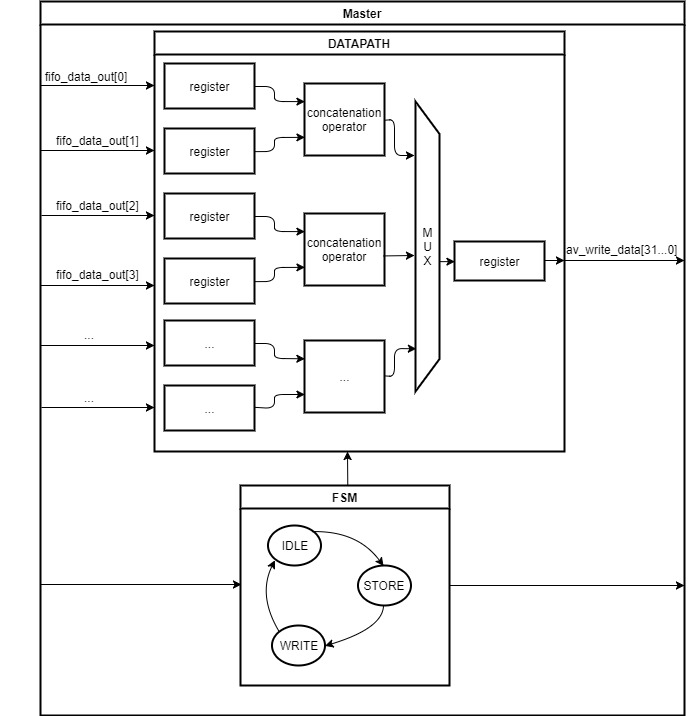
\includegraphics[scale=0.6]{images/MasterInside.png}
\caption{Master --- Internal structure of the datapath}
\label{fig:MasterInside}
\end{figure}

\subsubsection{Timing}

The same timings as presented in theory were observed in the results of Modelsim simulations and also with the logic analyzer. In the theoretical we made a mistake on the \verb'byte_enable'signal. Since we send 32-bit words in parallel, all the bytes are assumed valid and thus \verb'byte_enable' should always  be \verb'1111' (The signal could even be ignored to our knowledge). Figures \ref{fig:MasterAvalonTiming} and \ref{fig:MasterFifoTiming} we show the simulation results of the master component working isolated from the rest of the design by providing arbitrary FIFO output signals as a stimuli.
\begin{figure}[H]
\centering
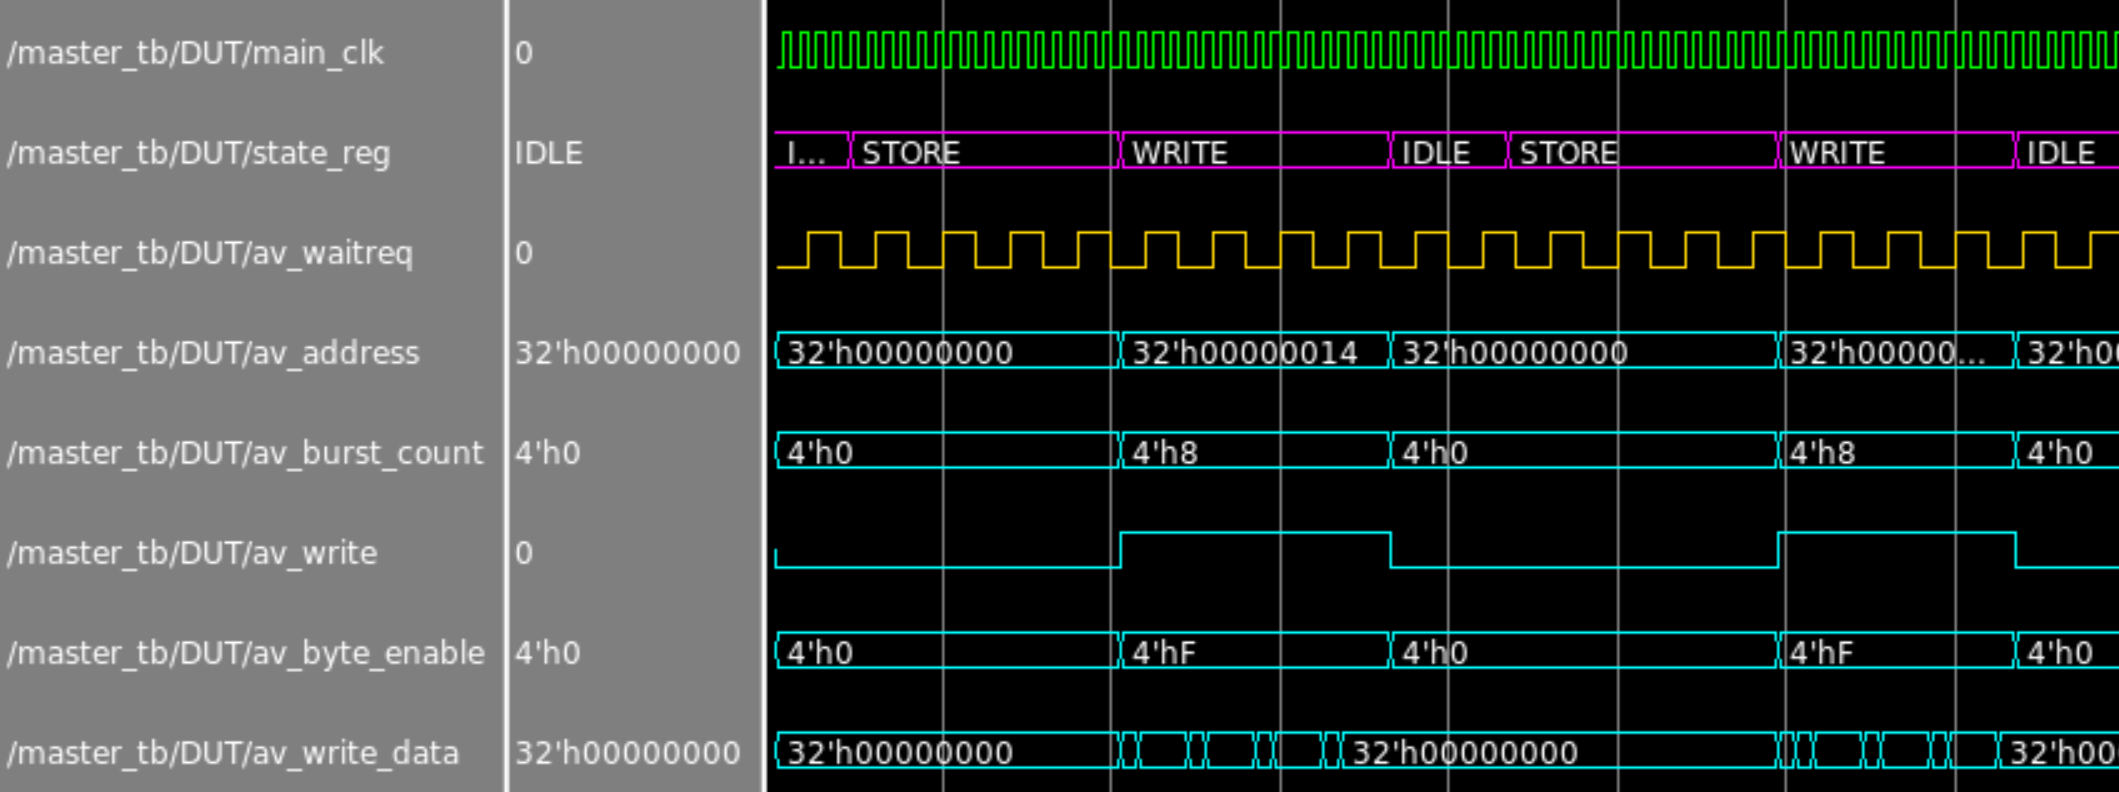
\includegraphics[scale=0.65]{images/MasterAvalonTiming.png}
\caption{Results of Modelsim simulation of master component --- Avalon signals}
\label{fig:MasterAvalonTiming}
\end{figure}

\begin{figure}[H]
\centering
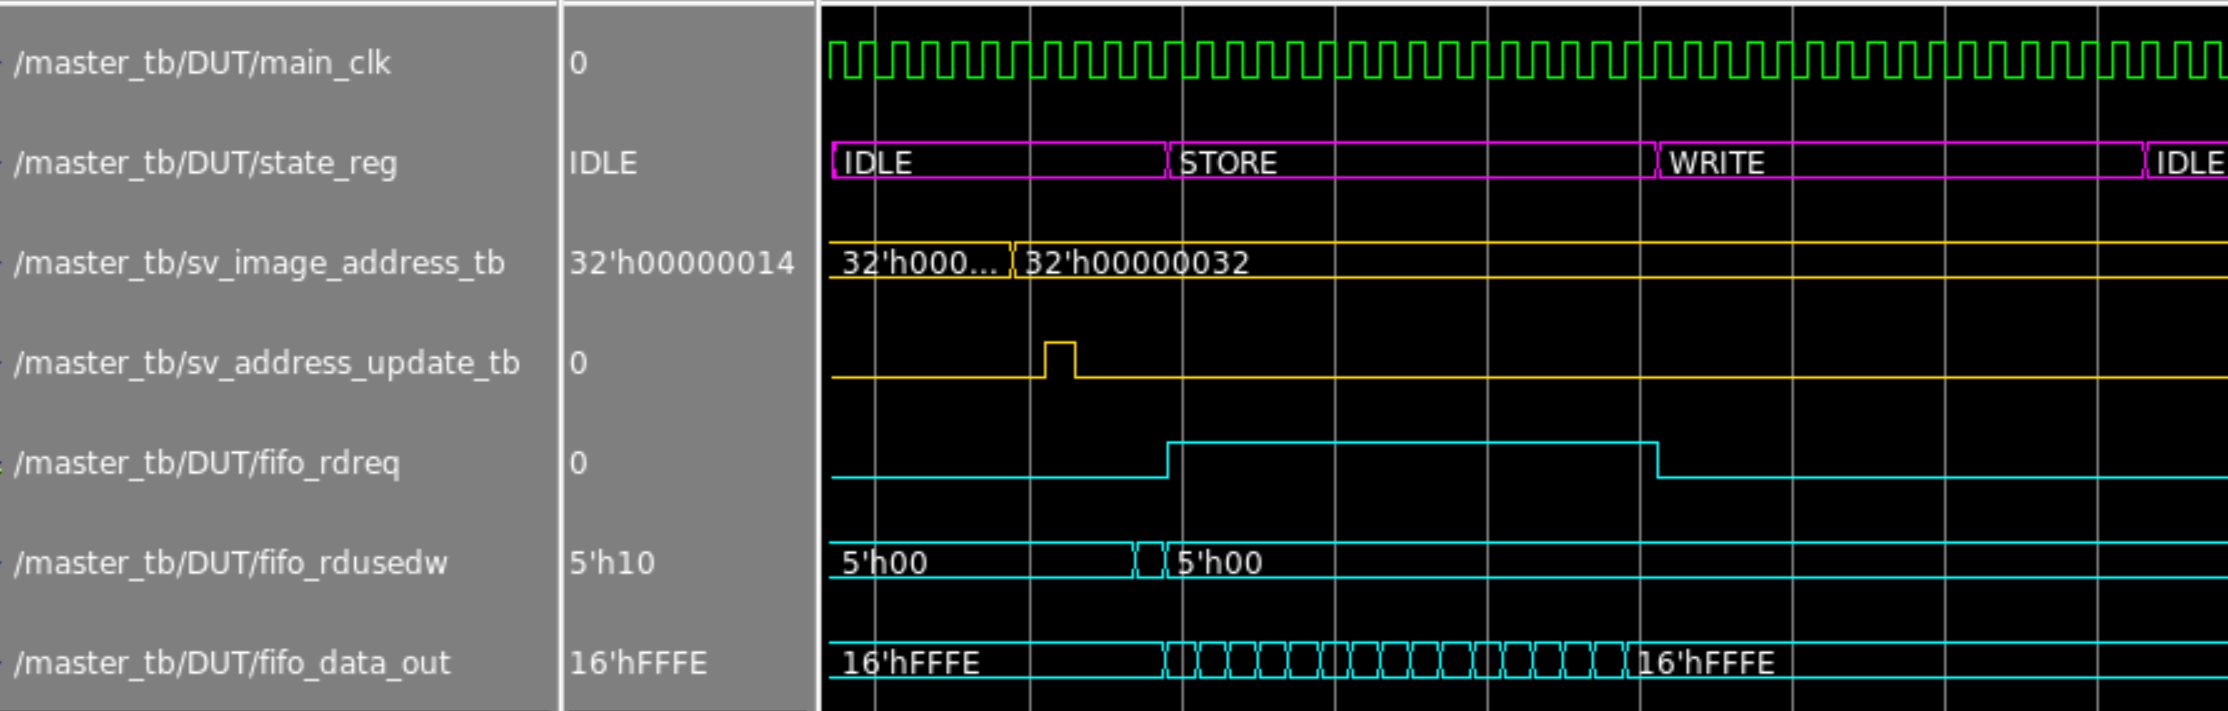
\includegraphics[scale=0.62]{images/MasterFifoTiming.png}
\caption{Results of Modelsim simulations of master component --- PixFIFO signals}
\label{fig:MasterFifoTiming}
\end{figure}

\subsection{Altera FIFO components configuration}
\subsection{Custom Component top-level Connection}
\section{Qsys Configuration and Interconnects}
\todo{Describe the use of PLL, I2C connections, address span expander, interrupt assignment, Custom component connections + ADD Qsys connections screen shot}

\section{Software programming of the NIOS II processor}

\todo{I'm not sure about the subtitles here, feel free to change or re-organize if you had another structure in mind}
\subsection{Camera configurations}
\subsection{Image dumping on a PC}
\subsection{Interfacing with an LCD}

\section{Errata}
\todo[inline]{
Buffer overrun if camera is not configured correctly (wrong image size). The DMA writes the whole data stream into memory without boundary check. \\
    
}

\section{Conclusion}

\end{document}
